%%%%%%%%%%%%%%%%%%%%%%%%%%%%%%%%%%%%%%%%%%%%%%%%%%%%%%%%%%
\begin{frame}
  \begin{center}
    {\Large Data Reading}
  \end{center}
\end{frame}

%%%%%%%%%%%%%%%%%%%%%%%%%%%%%%%%%%%%%%%%%%%%%%%%%%%%%%%%%%%%%%%%%%%%%%%%%%%%%%%%%%
\begin{frame}[fragile]\frametitle{Getting Data}
\begin{itemize}
\item In order to be a data scientist you need data.
\item Most of the time you are  acquiring, cleaning, and transforming data. 
\item Will see ways to acquire data, first
\end{itemize}
\end{frame}


%%%%%%%%%%%%%%%%%%%%%%%%%%%%%%%%%%%%%%%%%%%%%%%%%%%%%%%%%%%%%%%%%%%%%%%%
\begin{frame}[fragile]\frametitle{Files I/O (Recap)}
\begin{lstlisting}
# 'r' means read-only
file_for_reading = open('reading_file.txt', 'r')

# 'w' is write -- will destroy the file if already exists!
file_for_writing = open('writing_file.txt', 'w')

# 'a' is append -- for adding to the end of the file
file_for_appending = open('appending_file.txt', 'a')

# don't forget to close your files when you're done
file_for_writing.close()
\end{lstlisting}
\end{frame}

%%
%%%%%%%%%%%%%%%%%%%%%%%%%%%%%%%%%%%%%%%%%%%%%%%%%%%%%%%%%%%%%%%%%%%%%%%%%%
%%\begin{frame}[fragile]\frametitle{Reading File (Recap)}
%%\begin{lstlisting}
%%def get_domain(email_address):
%%    """split on '@' and return the last piece"""
%%    return email_address.lower().split("@")[-1]
%%    
%%with open('email_addresses.txt', 'r') as f:
%%    domain_counts = Counter(get_domain(line.strip())
%%                            for line in f
%%                            if "@" in line)
%%\end{lstlisting}
%%\end{frame}

%%%%%%%%%%%%%%%%%%%%%%%%%%%%%%%%%%%%%%%%%%%%%%%%%%%%%%%%%%%%%%%%%%%%%%%%%%
%%\begin{frame}[fragile]\frametitle{Reading File (Recap)}
%%\begin{lstlisting}
%%def get_domain(email_address):
%%    """split on '@' and return the last piece"""
%%    return email_address.lower().split("@")[-1]
%%    
%%with open('email_addresses.txt', 'r') as f:
%%    domain_counts = Counter(get_domain(line.strip())
%%                            for line in f
%%                            if "@" in line)
%%\end{lstlisting}
%%\end{frame}

%%%%%%%%%%%%%%%%%%%%%%%%%%%%%%%%%%%%%%%%%%%%%%%%%%%%%%%%%%%%%%%%%%%%%%%%
\begin{frame}[fragile]\frametitle{Assignment: Reading File}
\begin{itemize}
\item Open 'tab\_delimited\_stock\_prices.txt'
\item Read using csv.reader from csv module
\item Print date, stock symbol and price
\end{itemize}
\end{frame}


%%%%%%%%%%%%%%%%%%%%%%%%%%%%%%%%%%%%%%%%%%%%%%%%%%%%%%%%%%%%%%%%%%%%%%%%
\begin{frame}[fragile]\frametitle{Solution: Reading File}
\begin{lstlisting}
with open('data/tab_delimited_stock_prices.txt', 'r') as f:
    reader = csv.reader(f, delimiter='\t')
    for row in reader:
        date = row[0]
        symbol = row[1]
        closing_price = float(row[2])
        print("Date {}, Stock {} Price{}".format(date, symbol, closing_price))
\end{lstlisting}

\begin{lstlisting}
Date 6/20/2014, Stock AAPL Price90.91
Date 6/20/2014, Stock MSFT Price41.68
Date 6/20/2014, Stock FB Price64.5
Date 6/19/2014, Stock AAPL Price91.86
Date 6/19/2014, Stock MSFT Price41.51
Date 6/19/2014, Stock FB Price64.34
\end{lstlisting}
\end{frame}

%%%%%%%%%%%%%%%%%%%%%%%%%%%%%%%%%%%%%%%%%%%%%%%%%%%%%%%%%%%%%%%%%%%%%%%%
\begin{frame}[fragile]\frametitle{Assignment: Reading File}
\begin{itemize}
\item Open 'colon\_delimited\_stock\_prices.txt'
\item Get each row as a  dict  (with the headers as keys) by using  csv.DictReader
\item Print date, stock symbol and price
\end{itemize}
\end{frame}


%%%%%%%%%%%%%%%%%%%%%%%%%%%%%%%%%%%%%%%%%%%%%%%%%%%%%%%%%%%%%%%%%%%%%%%%
\begin{frame}[fragile]\frametitle{Solution: Reading File}
\begin{lstlisting}
    reader = csv.DictReader(f, delimiter=':')
    for row in reader:
        date = row["date"]
        symbol = row["symbol"]
        closing_price = float(row["closing_price"])
        print("Date {}, Stock {} Price {}".format(date, symbol, closing_price))
\end{lstlisting}
\begin{lstlisting}
Date 6/20/2014, Stock AAPL Price 90.9
Date 16/20/2014, Stock MSFT Price 41.68
Date 6/20/2014, Stock FB Price 64.5
\end{lstlisting}
\end{frame}


%%%%%%%%%%%%%%%%%%%%%%%%%%%%%%%%%%%%%%%%%%%%%%%%%%%%%%%%%%
\begin{frame}[fragile]\frametitle{Data Preprocessing}	
\begin{itemize}
\item Data Exploration phase results in finding data quality issues. Outliers, missing values
\item Feature Engineering is the way to prepare data.

\end{itemize}
\end{frame}


%%%%%%%%%%%%%%%%%%%%%%%%%%%%%%%%%%%%%%%%%%%%%%%%%%%%%%%%%%
\begin{frame}
  \begin{center}
    {\Large Feature Engineering}
  \end{center}
\end{frame}



%%%%%%%%%%%%%%%%%%%%%%%%%%%%%%%%%%%%%%%%%%%%%%%%%%%%%%%%%%%
\begin{frame}[fragile]\frametitle{The Art of Feature Engineering}
What is Feature Engineering? 
	\begin{itemize}
	\item The science (and art) of extracting more information from existing data. 
\item E.g. To predict footfall in a mall, if you collect data date wise, it may not have meaningful insight, but if you collect day-of-the-week wise, may get some patterns.
\item This is done as part of Data Preparation, before doing Machine Learning modeling.
	\end{itemize}
\end{frame}

%%%%%%%%%%%%%%%%%%%%%%%%%%%%%%%%%%%%%%%%%%%%%%%%%%%%%%%%%%%
\begin{frame}[fragile]\frametitle{The Art of Feature Engineering}
What is the process of Feature Engineering ? 
	\begin{itemize}
	\item Variable transformation. 
	\item Variable / Feature creation. 
	\end{itemize}
\end{frame}


%%%%%%%%%%%%%%%%%%%%%%%%%%%%%%%%%%%%%%%%%%%%%%%%%%%%%%%%%%%
\begin{frame}[fragile]\frametitle{The Art of Feature Engineering}
What is Variable Transformation? 
	\begin{itemize}
	\item  refers to the replacement of a variable by a function.
\item For 
instance, replacing a variable x by the square / cube root or logarithm x is a transformation.

	\end{itemize}
\end{frame}


%%%%%%%%%%%%%%%%%%%%%%%%%%%%%%%%%%%%%%%%%%%%%%%%%%%%%%%%%%%
\begin{frame}[fragile]\frametitle{The Art of Feature Engineering}
What are the common methods of Variable Transformation? 
	\begin{itemize}
	\item logarithm: skewed distribution to normal
	\item sq root, cube root
	\item Binning
	\item Change the scale
\item  Transform complex non-linear relationships into linear relationships
	\end{itemize}
	
	
\end{frame}


%%%%%%%%%%%%%%%%%%%%%%%%%%%%%%%%%%%%%%%%%%%%%%%%%%%%%%%%%%
\begin{frame}
  \begin{center}
    {\Large Data Processing: Variable Transformations}
  \end{center}
\end{frame}



%%%%%%%%%%%%%%%%%%%%%%%%%%%%%%%%%%%%%%%%%%%%%%%%%%%%%%%%%%%%%%%%%%%%%%%%
\begin{frame}[fragile]\frametitle{PreProcessing Techniques}
Changing the way data is represented just to make it more compatible with certain machine learning algorithms:

\begin{itemize}
\item Scaling: Normalization, Standardization 
\item Missing value replacement
\item Binning 
\item Sampling 
\item Feature Selection
\item Dimensionality Reduction: PCA
\item Encoding
\end{itemize}
\end{frame}


%%%%%%%%%%%%%%%%%%%%%%%%%%%%%%%%%%%%%%%%%%%%%%%%%%%%%%%%%%
\begin{frame}
  \begin{center}
    {\Large Scaling}
  \end{center}
\end{frame}

%%%%%%%%%%%%%%%%%%%%%%%%%%%%%%%%%%%%%%%%%%%%%%%%%%%%%%%%%%
\begin{frame}[fragile]\frametitle{Normalization}	
Typical ranges used for normalizing feature values are [0,1] and [-1,1].

\begin{itemize}
\item Change a continuous feature to fall within a specified range while maintaining the relative differences between the values for the feature
\item Example:
Customer ages in a data-set: [16, 96]
Customer salaries: [10000, 100000]
\item Range Normalization: convert a feature value into the range [low , high] 
\item Re-parametrization to the new range.
\end{itemize}
Sensitive to the presence of Outliers in a data-set.
\end{frame}

%%%%%%%%%%%%%%%%%%%%%%%%%%%%%%%%%%%%%%%%%%%%%%%%%%%%%%%%%%%%%%%%%%%%%%%%
\begin{frame}[fragile]\frametitle{Sklearn Normalization}
% Normalization: To transform data the [0,1] range. Done by removing min value from all and then dividing by length (max-min).
	\begin{itemize}
	\item Use function sklearn.preprocessing.normalize()
	\item  X: Data to be normalized
	\item norm: which norm to use: l1 (sum of elements gives 1) or l2 (sqrt the sum of the squares of the elements gives one)
	\item axis: whether to normalize by row or column
	\end{itemize}
\end{frame}






%%%%%%%%%%%%%%%%%%%%%%%%%%%%%%%%%%%%%%%%%%%%%%%%%%%%%%%%%%%%%%%%%%%%%%%%
\begin{frame}[fragile]\frametitle{Standardization}
Standardization: To transform data so that it has zero mean and unit variance. Also called scaling.
Done by removing the mean value from all points, then scale it by dividing with the standard deviation.
	\begin{itemize}
	\item Use function sklearn.preprocessing.scale()
	\item  X: Data to be scaled.
	\item with\_mean: Boolean. Make zero mean or not.
	\item with\_std: Make unit standard deviation or not.
	\end{itemize}
\end{frame}



%%%%%%%%%%%%%%%%%%%%%%%%%%%%%%%%%%%%%%%%%%%%%%%%%%%%%%%%%%
\begin{frame}[fragile]\frametitle{Standardization}	
Majority of feature values will be in a range of [-1, 1].

\begin{itemize}
\item Measures how many standard deviations a feature value is from the mean for that feature
\item  Mean = 0, Standard deviation = 1 
\item  $Standard Scores = a'_i = \frac{a_i - \bar{a}}{sd(a)}$
\end{itemize}
Standardization assumes the feature values are normally distributed. If not, standardization may introduce some distortions.

\end{frame}


%%%%%%%%%%%%%%%%%%%%%%%%%%%%%%%%%%%%%%%%%%%%%%%%%%%%%%%%%%
\begin{frame}[fragile]\frametitle{Example}	
\begin{center}
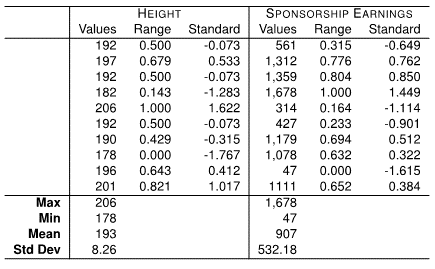
\includegraphics[width=0.8\linewidth,keepaspectratio]{stdex}
\end{center}
\end{frame}

%%%%%%%%%%%%%%%%%%%%%%%%%%%%%%%%%%%%%%%%%%%%%%%%%%%%%%%%%%%%%%%%%%%%%%%%
\begin{frame}[fragile]\frametitle{Sklearn Standardization/Scaling}
\begin{lstlisting}
from sklearn import preprocessing
import numpy as np

X = np.array([[ 1., -1.,  2.],
				 [ 2.,  0.,  0.],
				[ 0.,  1., -1.]])
				
X_scaled = preprocessing.scale(X)

print(X_scaled)

array([[ 0.  ..., -1.22...,  1.33...],
       [ 1.22...,  0.  ..., -0.26...],
       [-1.22...,  1.22..., -1.06...]])
\end{lstlisting}
\end{frame}


%%%%%%%%%%%%%%%%%%%%%%%%%%%%%%%%%%%%%%%%%%%%%%%%%%%%%%%%%%
\begin{frame}
  \begin{center}
    {\Large Binning}
  \end{center}
\end{frame}


%%%%%%%%%%%%%%%%%%%%%%%%%%%%%%%%%%%%%%%%%%%%%%%%%%%%%%%%%%
\begin{frame}[fragile]\frametitle{Binning}	
\begin{itemize}
\item Converting a continuous feature into a categorical feature
\item Define a series of ranges (called bins) for the continuous feature that correspond to the levels of the new categorical feature
\item Approaches: 
	\begin{itemize}
	\item equal-width binning 
	\item equal-frequency binning 
	\end{itemize}
\item Need to ``manually'' decide the number of bins:
	\begin{itemize}
	\item Choosing a low number may lose a lot of information
	\item Choosing a very high number might result in a very few instances in each bin or empty bins
	\end{itemize}
\end{itemize}
\end{frame}

%%%%%%%%%%%%%%%%%%%%%%%%%%%%%%%%%%%%%%%%%%%%%%%%%%%%%%%%%%
\begin{frame}[fragile]\frametitle{Binning}	
\begin{center}
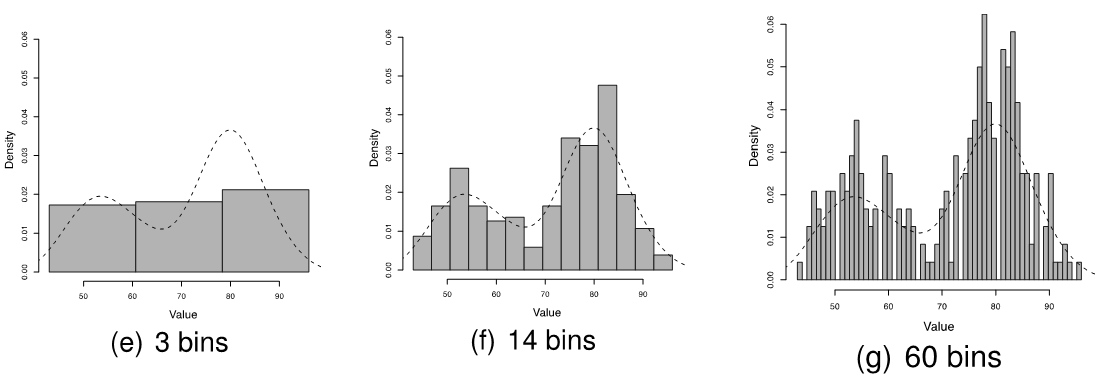
\includegraphics[width=\linewidth,keepaspectratio]{bins}
\end{center}
\end{frame}

%%%%%%%%%%%%%%%%%%%%%%%%%%%%%%%%%%%%%%%%%%%%%%%%%%%%%%%%%%
\begin{frame}[fragile]\frametitle{Equal-Width Binning}	
\begin{itemize}
\item Splits the range of the feature values into b bins each of size $\frac{range}{b}$
\item Usually works well
\item Some near-empty bins when data follows a normal distribution
\end{itemize}
\end{frame}


%%%%%%%%%%%%%%%%%%%%%%%%%%%%%%%%%%%%%%%%%%%%%%%%%%%%%%%%%%
\begin{frame}[fragile]\frametitle{Equal-Width Binning}	
\begin{center}
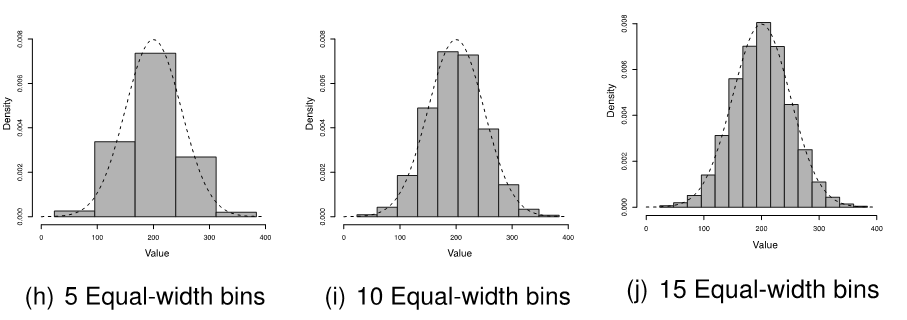
\includegraphics[width=\linewidth,keepaspectratio]{eqbins}
\end{center}
\end{frame}


%%%%%%%%%%%%%%%%%%%%%%%%%%%%%%%%%%%%%%%%%%%%%%%%%%%%%%%%%%
\begin{frame}[fragile]\frametitle{Equal-Frequency Binning}	
\begin{itemize}
\item Algorithm:
	\begin{itemize}
	\item Sorts the continuous feature values into ascending order 
	\item Then places an equal number of instances into each bin, starting with bin 1 
	\end{itemize}
\item Number of instances placed in each bin $\frac{TotalNumberOfInstances}{NumberOfBins}$
\end{itemize}
\end{frame}


%%%%%%%%%%%%%%%%%%%%%%%%%%%%%%%%%%%%%%%%%%%%%%%%%%%%%%%%%%
\begin{frame}[fragile]\frametitle{Equal-Frequency Binning}	
\begin{center}
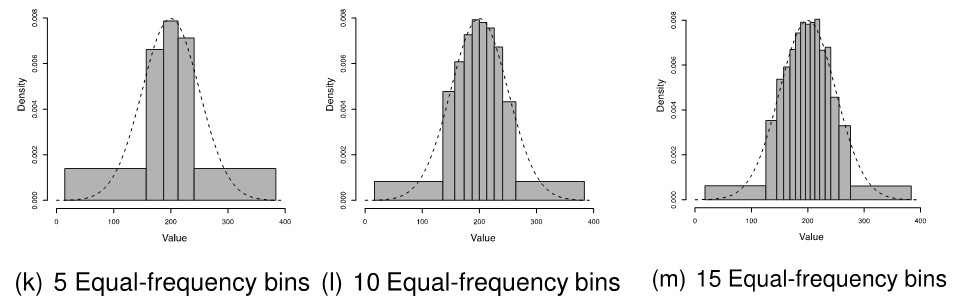
\includegraphics[width=\linewidth,keepaspectratio]{eqfrqbins}
\end{center}
\end{frame}

%%%%%%%%%%%%%%%%%%%%%%%%%%%%%%%%%%%%%%%%%%%%%%%%%%%%%%%%%%
\begin{frame}[fragile]\frametitle{Data Preparation: Sampling}	
\begin{itemize}
\item Sometimes we have too much data!, instead sample a smaller percentage from the larger dataset
\item Care required when sampling:
	\begin{itemize}
	\item Try to ensure that the resulting datasets is still representative of the original data and that no unintended bias is introduced during this process. 
	\item If not, any modeling on the sample will not be relevant to the overall dataset.
	\end{itemize}
\end{itemize}
\end{frame}

%%%%%%%%%%%%%%%%%%%%%%%%%%%%%%%%%%%%%%%%%%%%%%%%%%%%%%%%%%
\begin{frame}[fragile]\frametitle{Data Preparation: Sampling}	
\begin{center}
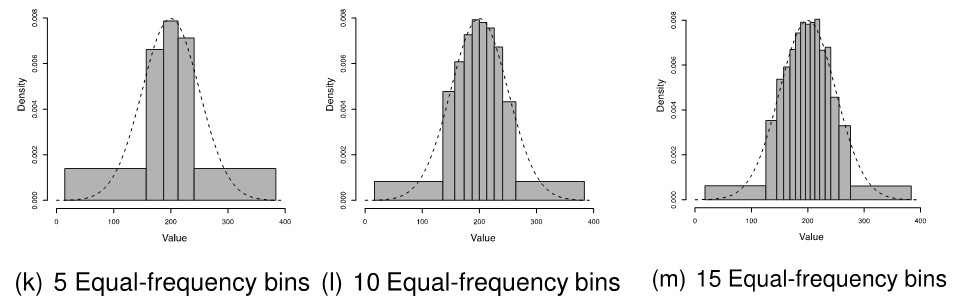
\includegraphics[width=\linewidth,keepaspectratio]{eqfrqbins}
\end{center}
\end{frame}


%%%%%%%%%%%%%%%%%%%%%%%%%%%%%%%%%%%%%%%%%%%%%%%%%%%%%%%%%%
\begin{frame}
  \begin{center}
    {\Large Handling Outliers}
  \end{center}
\end{frame}



%%%%%%%%%%%%%%%%%%%%%%%%%%%%%%%%%%%%%%%%%%%%%%%%%%%%%%%%%%
\begin{frame}[fragile]\frametitle{Clamp Transformation}	
\begin{itemize}
\item Clamps all values above an upper threshold and below a lower threshold to remove outliers
\item Upper and lower thresholds can be set manually based on domain knowledge
\item Or:
\begin{itemize}
\item Lower = 1st quartile -1.5 x inter-quartile range
\item Upper = 3rd quartile + 1.5 x inter-quartile range
\end{itemize}
\item Lower and upper are the specific thresholds.
\end{itemize}
\end{frame}

%%%%%%%%%%%%%%%%%%%%%%%%%%%%%%%%%%%%%%%%%%%%%%%%%%%%%%%%%%
\begin{frame}[fragile]\frametitle{Case Study: Outliers}	
Data quality issues found in the motor Insurance fraud dataset
\begin{center}
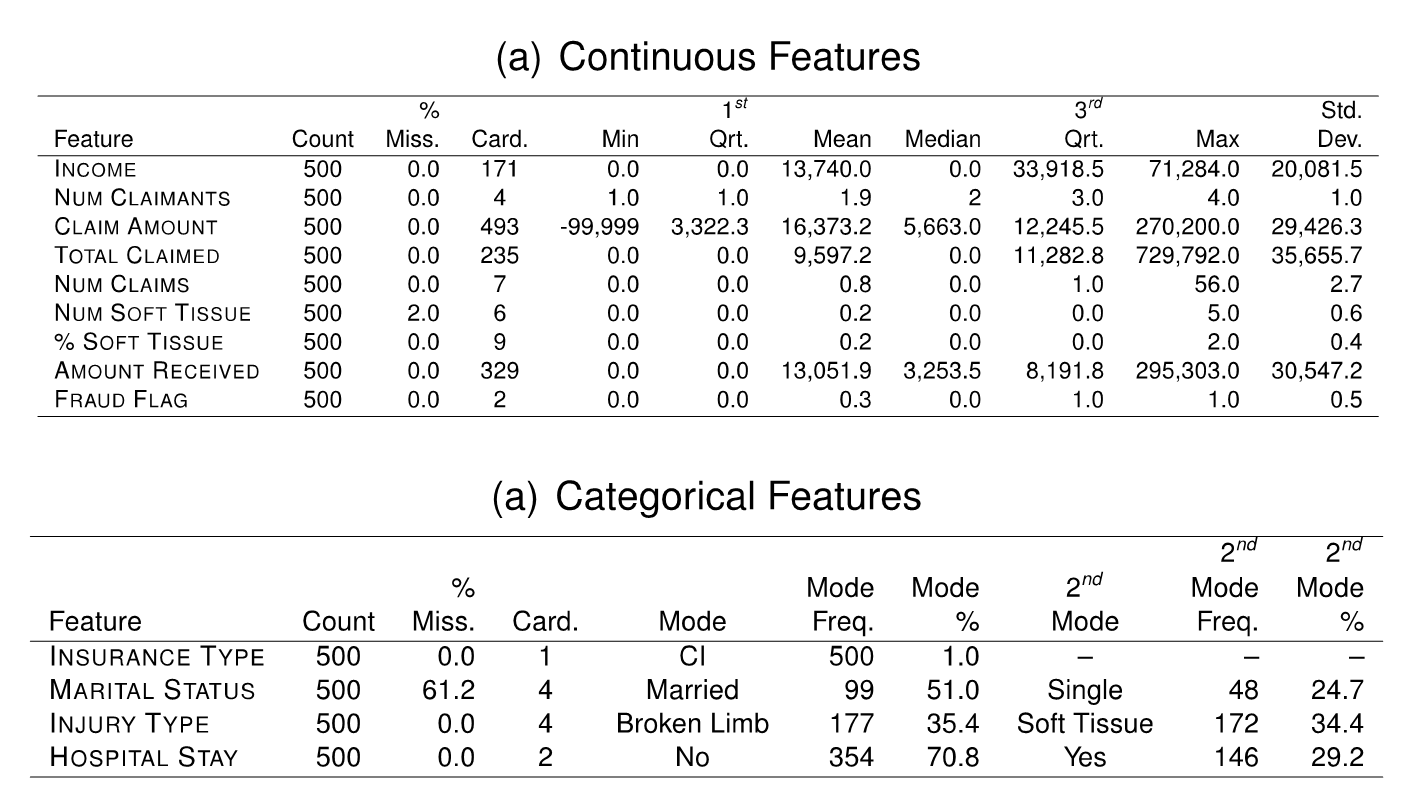
\includegraphics[width=\linewidth,keepaspectratio]{insurance}
\end{center}
\end{frame}

%%%%%%%%%%%%%%%%%%%%%%%%%%%%%%%%%%%%%%%%%%%%%%%%%%%%%%%%%%
\begin{frame}
  \begin{center}
    {\Large Handling Missing Value}
  \end{center}
\end{frame}



%%%%%%%%%%%%%%%%%%%%%%%%%%%%%%%%%%%%%%%%%%%%%%%%%%%%%%%%%%
\begin{frame}[fragile]\frametitle{Handling Missing Data}	
	\begin{itemize}
	\item Motivation: We will frequently encounter missing values, especially in big data. Lots of fields, lots of observations
	\item Question: how to handle the missing data?
	\end{itemize}

\end{frame}

%%%%%%%%%%%%%%%%%%%%%%%%%%%%%%%%%%%%%%%%%%%%%%%%%%%%%%%%%%
\begin{frame}[fragile]\frametitle{How much data is missing?}	
\begin{itemize}
\item Handling Missing Data:
	\begin{itemize}
	\item Dataset of 30 variables
	\item 5\% of data is missing
	\item Missing values are spread evenly throughout data
	\end{itemize}
\item 80\% of records would have at least one missing value
\item Bad solution: Deleting records with any missing data
\end{itemize}
\end{frame}

%%%%%%%%%%%%%%%%%%%%%%%%%%%%%%%%%%%%%%%%%%%%%%%%%%%%%%%%%%
\begin{frame}[fragile]\frametitle{Handling Missing Values (Dropping)}	
\begin{itemize}
\item Drop any features that have missing values. Might lead to massive loss of data
\item Drop any instance/record that has a missing value. Might lead to bias
\item Derive a missing indicator feature from features with missing values. Replace with a binary feature, whether the value was missing or not.
\item Ignore missing values. If data mining method is robust
\end{itemize}
\end{frame}

%%%%%%%%%%%%%%%%%%%%%%%%%%%%%%%%%%%%%%%%%%%%%%%%%%%%%%%%%%
\begin{frame}[fragile]\frametitle{Handling Missing Values (Imputation)}	
\begin{itemize}
\item Replace missing value with some constant (Specified by analyst)
\item Replace missing value with mean, median, or mode
\item Replace missing value with value generated at random from the observed variable distribution
\item Replace missing value with imputed values, based on other characteristics of the record
\end{itemize}
\end{frame}

%%%%%%%%%%%%%%%%%%%%%%%%%%%%%%%%%%%%%%%%%%%%%%%%%%%%%%%%%%%%%%%%%%%%%%%%
\begin{frame}[fragile]
\frametitle{Data Frames: Missing Values}
Missing values are marked as NaN

\begin{lstlisting}
# Read a dataset with missing values
flights = pd.read_csv("http://rcs.bu.edu/examples/python/data_analysis/flights.csv")

# Select the rows that have at least one missing value
flights[flights.isnull().any(axis=1)].head()
\end{lstlisting}
\begin{center}
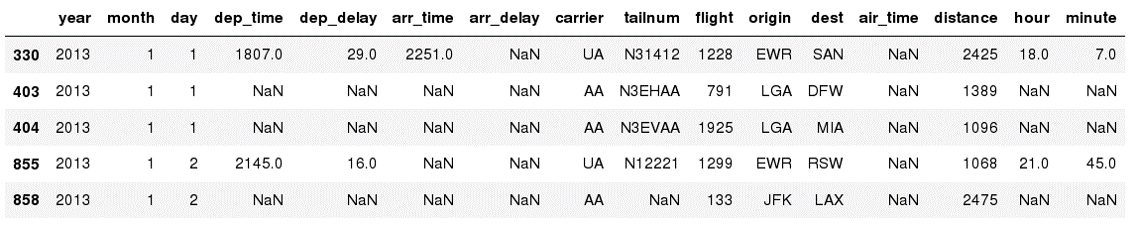
\includegraphics[width=\linewidth,keepaspectratio]{pdf9}
\end{center}
\end{frame}

%%%%%%%%%%%%%%%%%%%%%%%%%%%%%%%%%%%%%%%%%%%%%%%%%%%%%%%%%%%%%%%%%%%%%%%%
\begin{frame}[fragile]
\frametitle{Data Frames: Missing Values}
There are a number of methods to deal with missing values in the data frame:
\begin{center}
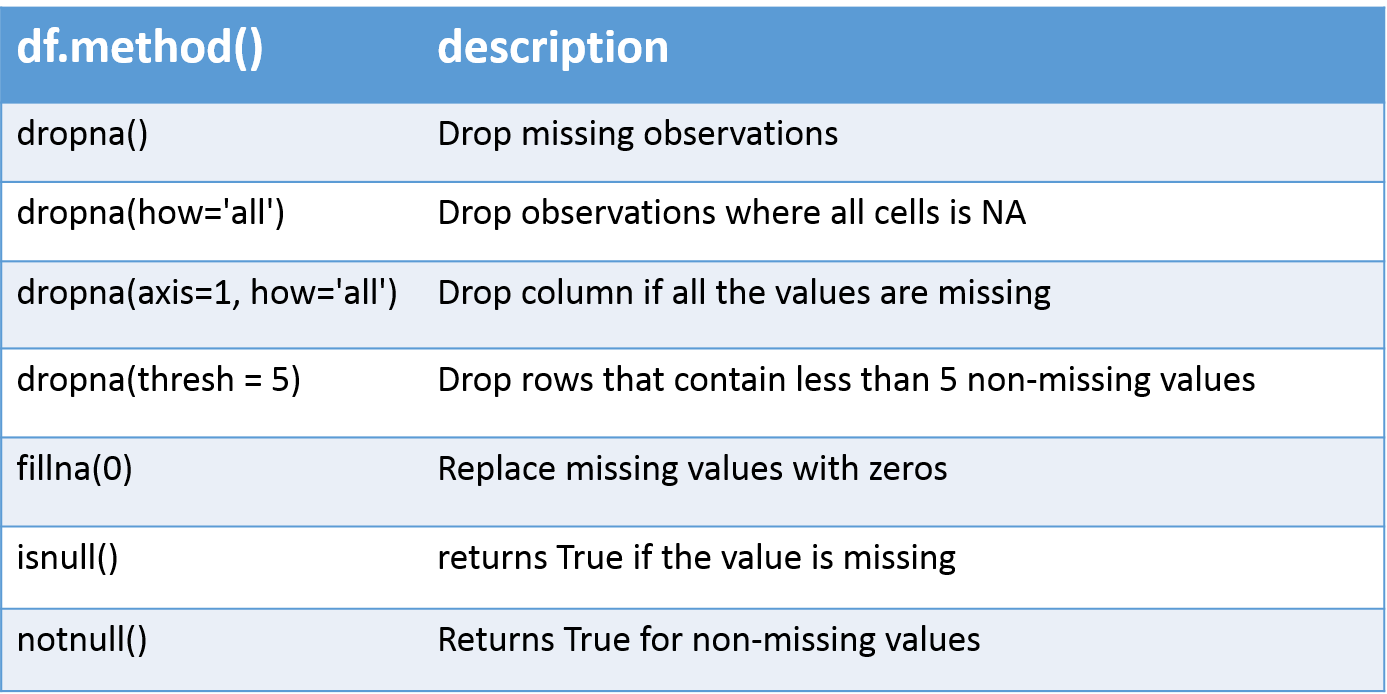
\includegraphics[width=\linewidth,keepaspectratio]{pdf10}
\end{center}
\end{frame}


%%%%%%%%%%%%%%%%%%%%%%%%%%%%%%%%%%%%%%%%%%%%%%%%%%%%%%%%%%%%%%%%%%%%%%%%
\begin{frame}[fragile]\frametitle{Missing Value Replacement}
In scikit-learn, this is referred to as``Imputation''
	\begin{itemize}
	\item Use function sklearn.preprocessing.Imputer
	\item  strategy: What to replace the missing value with: mean / median / most\_frequent
	\item axis: Boolean. Whether to replace along rows or columns
	\end{itemize}
\end{frame}

%%%%%%%%%%%%%%%%%%%%%%%%%%%%%%%%%%%%%%%%%%%%%%%%%%%%%%%%%%%%%%%%%%%%%%%%
\begin{frame}[fragile]\frametitle{Example code for Replacing Missing Values}
\begin{lstlisting}
import numpy as np
from sklearn.preprocessing import Imputer

X = np.array([[23.56],[53.45],['NaN'],[44.44],[77.78],['NaN'],[234.44],[11.33],[79.87]])

print(X)

imp = Imputer(missing_values='NaN', strategy='mean', axis=0)
X = imp.fit_transform(X)

print(X)
\end{lstlisting}
\end{frame}

%%%%%%%%%%%%%%%%%%%%%%%%%%%%%%%%%%%%%%%%%%%%%%%%%%%%%%%%%%
\begin{frame}
  \begin{center}
    {\Large Encoding}
  \end{center}
\end{frame}

%%%%%%%%%%%%%%%%%%%%%%%%%%%%%%%%%%%%%%%%%%%%%%%%%%%%%%%%%%%%%%%%%%%%%%%%
\begin{frame}[fragile]\frametitle{Encoding}
	\begin{itemize}
	\item Scikit-learn doesn't directly handle categorical attributes well.
	\item In order to use them in the dataset, some sort of encoding needs to be performed.
	\item One good way to encode categorical attributes: if there are n categories, create n dummy binary variables representing each category.
	\item Can be done easily using the sklearn.preprocessing.oneHotEncoder class.
	\end{itemize}
\end{frame}

%%%%%%%%%%%%%%%%%%%%%%%%%%%%%%%%%%%%%%%%%%%%%%%%%%%%%%%%%%%%%%%%%%%%%%%%
\begin{frame}[fragile]\frametitle{Encoding}
\begin{lstlisting}
raw_data = {'first_name': ['Jason', 'Molly', 'Tina', 'Jake', 'Amy'], 
        'last_name': ['Miller', 'Jacobson', 'Ali', 'Milner', 'Cooze'], 
        'age': [42, 52, 36, 24, 73], 
        'city': ['San Francisco', 'Baltimore', 'Miami', 'Douglas', 'Boston']}
df = pd.DataFrame(raw_data, columns = ['first_name', 'last_name', 'age', 'city'])
\end{lstlisting}
\begin{center}
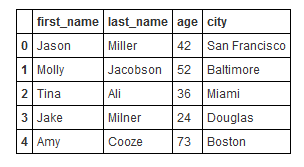
\includegraphics[width=0.4\linewidth]{dfcity1}
\end{center}
\end{frame}

%%%%%%%%%%%%%%%%%%%%%%%%%%%%%%%%%%%%%%%%%%%%%%%%%%%%%%%%%%%%%%%%%%%%%%%%
\begin{frame}[fragile]\frametitle{Encoding}
Convert Categorical Feature Into Dummy Variables Using Pandas
\begin{lstlisting}
pd.get_dummies(df["city"])
\end{lstlisting}
\begin{center}
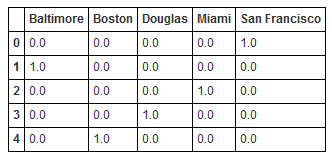
\includegraphics[width=0.6\linewidth]{dfcity2}
\end{center}
\end{frame}

%%%%%%%%%%%%%%%%%%%%%%%%%%%%%%%%%%%%%%%%%%%%%%%%%%%%%%%%%%%%%%%%%%%%%%%%
\begin{frame}[fragile]\frametitle{Encoding}
Convert Categorical Data Into OneHot Using Scikit
\begin{lstlisting}
integerized_data = preprocessing.LabelEncoder().fit_transform(df["city"])

preprocessing.OneHotEncoder().fit_transform(integerized_data.reshape(-1,1)).toarray()

array([[ 0.,  0.,  0.,  0.,  1.],
       [ 1.,  0.,  0.,  0.,  0.],
       [ 0.,  0.,  0.,  1.,  0.],
       [ 0.,  0.,  1.,  0.,  0.],
       [ 0.,  1.,  0.,  0.,  0.]])
\end{lstlisting}
\end{frame}

%%%%%%%%%%%%%%%%%%%%%%%%%%%%%%%%%%%%%%%%%%%%%%%%%%%%%%%%%%%%%%%%%%%%%%%%
\begin{frame}[fragile]\frametitle{Imp Note}
	\begin{itemize}
	\item All pre-processing steps done on X of training have to be done on X of testing also.
	\item Once results are predicted, you many need to reverse transform some of the features to find corresponding points in the original X.
	\end{itemize}
\end{frame}



%%%%%%%%%%%%%%%%%%%%%%%%%%%%%%%%%%%%%%%%%%%%%%%%%%%%%%%%%%
\begin{frame}
  \begin{center}
    {\Large Handling Intra Dependence}
  \end{center}
\end{frame}


%%%%%%%%%%%%%%%%%%%%%%%%%%%%%%%%%%%%%%%%%%%%%%%%%%%
\begin{frame}[fragile] \frametitle{Covariance}

\begin{itemize}
\item Visual preliminary exploration, comparing two variables, using scatter plots
\item Quantitative preliminary exploration using covariance and correlation measures
\item Covariance: $cov(a,b) = 1/(n-1) \sum ((a_i - \bar{a}) \times (b_i - \bar{b}))$

\end{itemize}


\begin{center}
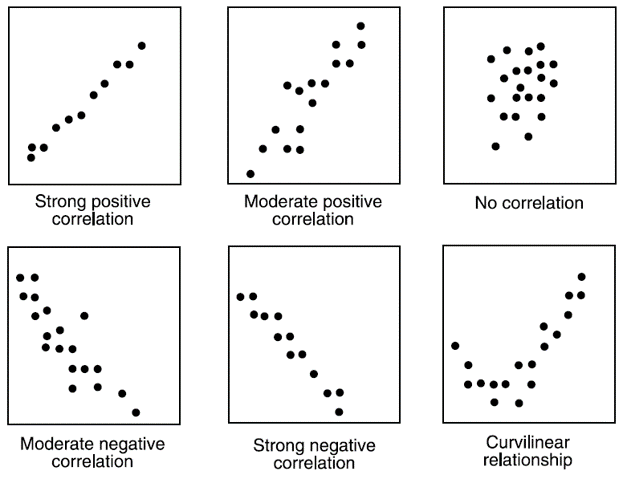
\includegraphics[width=0.6\linewidth,keepaspectratio]{cov}
\end{center}

\end{frame}


%%%%%%%%%%%%%%%%%%%%%%%%%%%%%%%%%%%%%%%%%%%%%%%%%%%
\begin{frame}[fragile] \frametitle{Covariance}

What is interesting in this data?

\begin{center}
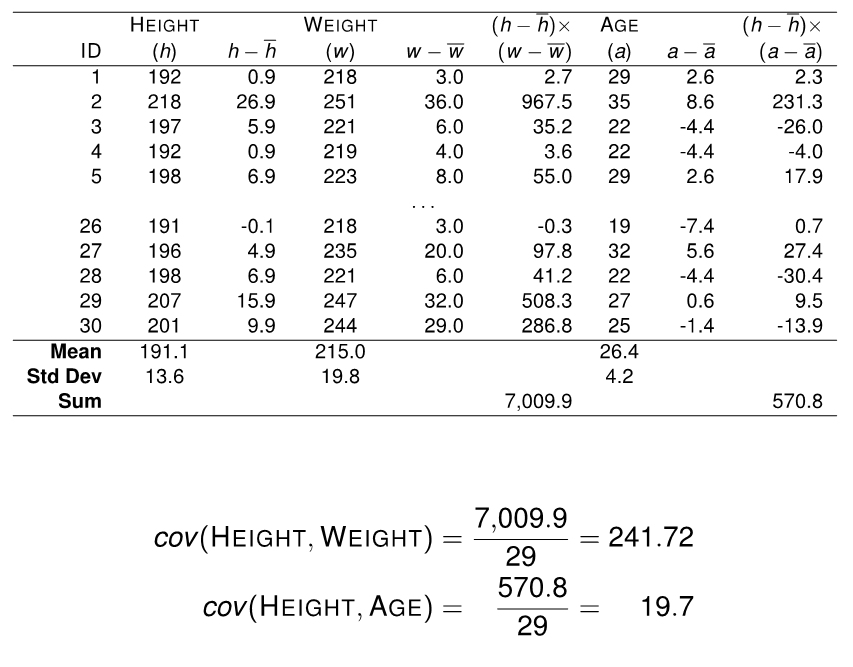
\includegraphics[width=0.7\linewidth,keepaspectratio]{covex}
\end{center}

\end{frame}


%%%%%%%%%%%%%%%%%%%%%%%%%%%%%%%%%%%%%%%%%%%%%%%%%%%
\begin{frame}[fragile] \frametitle{Covariance}

\begin{itemize}
\item Values fall into the range $[- \infty, \infty]$
\item Negative values indicate a negative relationship
\item Positive values indicate a positive relationship
\item Values near zero indicate that there is little or no relationship between the features
\item Calculating covariance between the HEIGHT feature and the WEIGHT and AGE features from the basketball players dataset
\end{itemize}

\end{frame}


%%%%%%%%%%%%%%%%%%%%%%%%%%%%%%%%%%%%%%%%%%%%%%%%%%%
\begin{frame}[fragile] \frametitle{Correlation}

\begin{center}
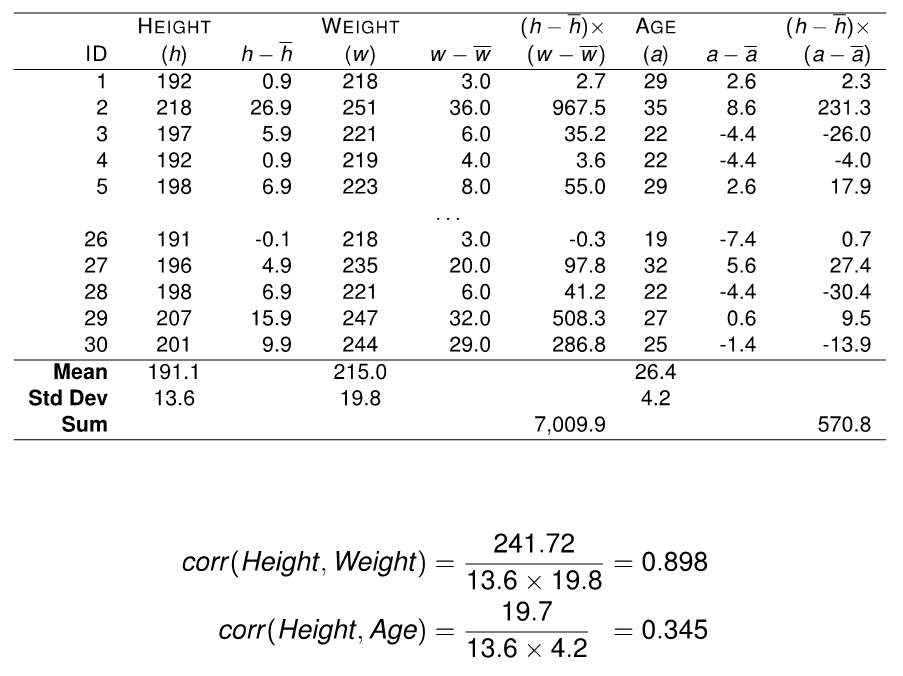
\includegraphics[width=0.8\linewidth,keepaspectratio]{corr}
\end{center}
\end{frame}



%%%%%%%%%%%%%%%%%%%%%%%%%%%%%%%%%%%%%%%%%%%%%%%%%%%
\begin{frame}[fragile] \frametitle{Correlation}

\begin{itemize}
\item Normalized form of covariance 
\item Values ranges between -1 and +1
\item Correlation: $corr(a,b) = \frac{cov(a,b)}{sd(a) \times sd(b)}$
\item values fall into the range [-1, 1]
\begin{itemize}
\item values close to -1 indicate a very strong negative correlation (or covariance)
\item values close to 1 indicate a very strong positive correlation
\item values around 0 indicate no correlation
\end{itemize}
\item Features that have no correlation are said to be independent. 
\item Calculating correlation between the HEIGHT feature and the WEIGHT and AGE features from the basketball players dataset. 
\end{itemize}
\end{frame}



%%%%%%%%%%%%%%%%%%%%%%%%%%%%%%%%%%%%%%%%%%%%%%%%%%%%%%%%%%
\begin{frame}[fragile]\frametitle{Covariance and Correlation Matrix}	
\begin{itemize}
\item There are usually multiple continuous features in a dataset to explore.
\item Covariance and Correlation Matrix for the display of every combination of features 
\end{itemize}
\begin{center}
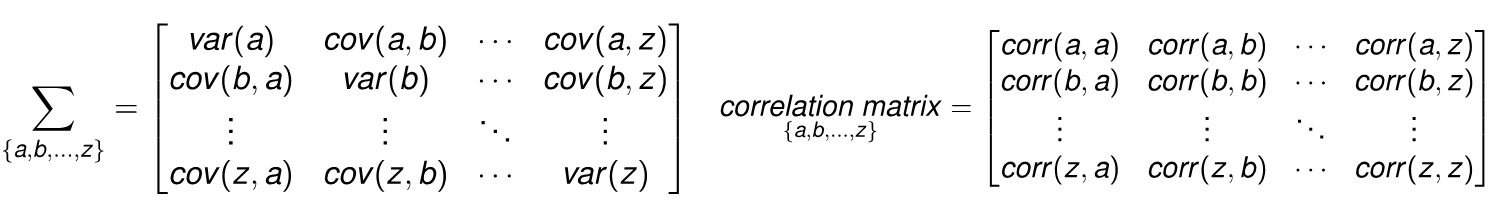
\includegraphics[width=\linewidth,keepaspectratio]{covcorr}
\end{center}
\end{frame}


%%%%%%%%%%%%%%%%%%%%%%%%%%%%%%%%%%%%%%%%%%%%%%%%%%%%%%%%%%
\begin{frame}[fragile]\frametitle{Example}	
\begin{center}
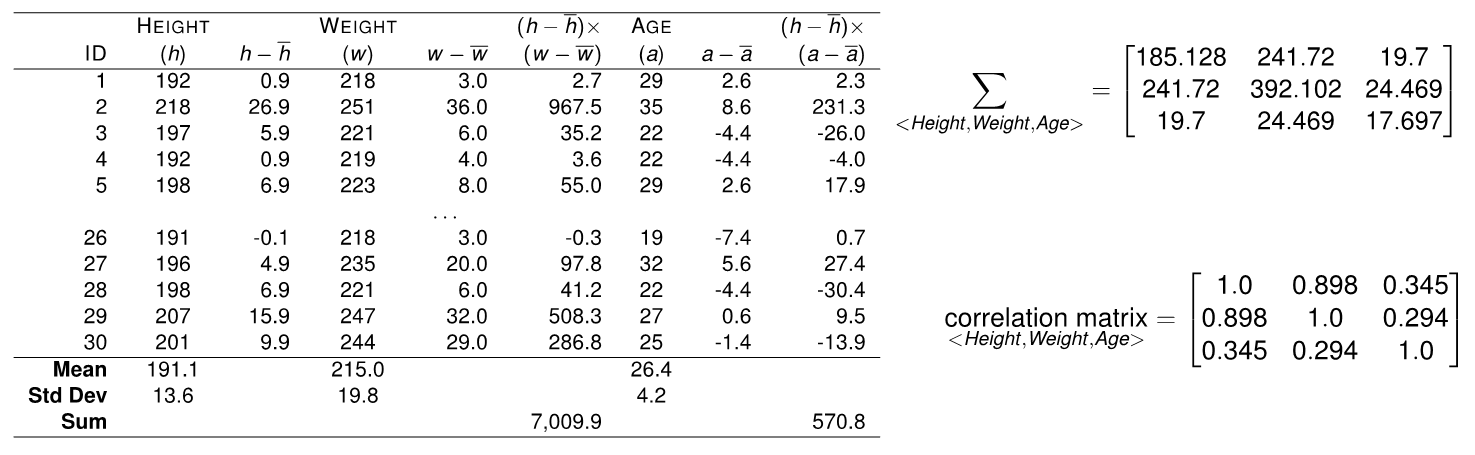
\includegraphics[width=\linewidth,keepaspectratio]{covcorrmat}
\end{center}
\end{frame}


%%%%%%%%%%%%%%%%%%%%%%%%%%%%%%%%%%%%%%%%%%%%%%%%%%%
\begin{frame}[fragile] \frametitle{Correlation does not Imply Causation}
\begin{center}
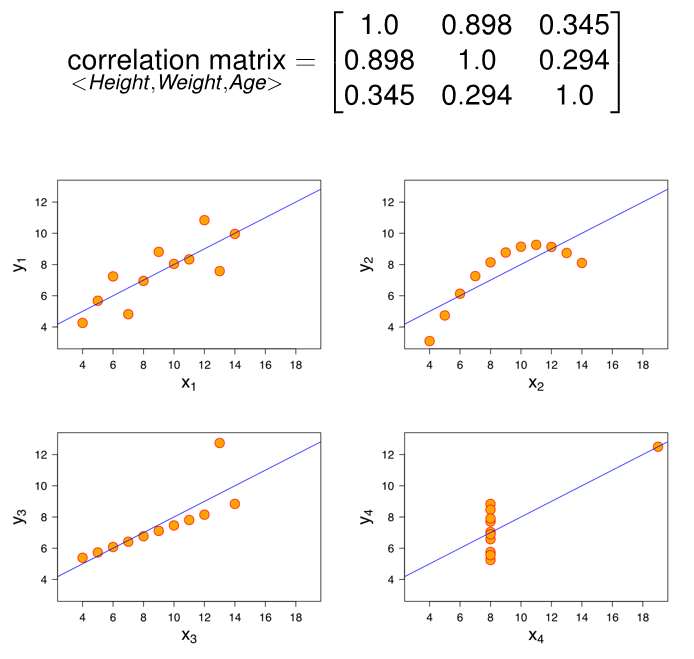
\includegraphics[width=0.5\linewidth,keepaspectratio]{corrcause}
\end{center}
\begin{itemize}
\item Correlation is a good measure of the relationship between two continuous features, but it is not by any means perfect.
\item  Still need visual analysis.
\end{itemize}
\end{frame}



%%%%%%%%%%%%%%%%%%%%%%%%%%%%%%%%%%%%%%%%%%%%%%%%%%%%%%%%%%
\begin{frame}[fragile]\frametitle{Correlation does not Imply Causation}	
Causation can be mistakenly assumed:

	\begin{itemize}
	\item Mistaking the order of a causal relationship
		\begin{itemize}
		\item Example: Spinning windmills cause wind.
		\item Example: Playing basketball causes people to be tall.
		\end{itemize}
	\item Inferring causation between two features while ignoring a third (hidden) feature.
		\begin{itemize}
		\item From Nature, 1999.
		\item ``causal relationship between young children sleeping with a night-light turned on and these children developing short-sightedness in later life''
		\item Short-sighted parents, because of poor night vision, tend to favor the use of night-lights; short-sighted parents are more likely to have short-sighted children.
		\end{itemize}
	\end{itemize}

\end{frame}





%%%%%%%%%%%%%%%%%%%%%%%%%%%%%%%%%%%%%%%%%%%%%%%%%%%%%%%%%%
\begin{frame}
  \begin{center}
    {\Large Data Processing: Variable Creation/Reduction}
  \end{center}
\end{frame}

%%%%%%%%%%%%%%%%%%%%%%%%%%%%%%%%%%%%%%%%%%%%%%%%%%%%%%%%%%%
\begin{frame}[fragile]\frametitle{The Art of Feature Engineering}
What is Feature / Variable Creation \& its Benefits? 
	\begin{itemize}
	\item Generate a new variables / features based on existing 
variable(s). 
\item For example, say, we have date(dd-mm-yy) as an input variable in a data set. We 
can  generate  new  variables  like  day,  month,  year,  week,  weekday  that  may  have  better 
relationship with target variable. 
	\end{itemize}

\begin{center}
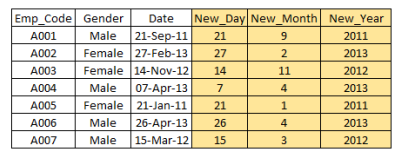
\includegraphics[width=0.8\linewidth,keepaspectratio]{eda10}
\end{center}
\end{frame}


%%%%%%%%%%%%%%%%%%%%%%%%%%%%%%%%%%%%%%%%%%%%%%%%%%%%%%%%%%%
\begin{frame}[fragile]\frametitle{Dealing with High Dimensionality}
	\begin{itemize}
	\item Feature Selection
	\item Feature Extraction
	\item Data Engineering: Processing, Assumptions
	\item Tree-based Approaches
	\item Factorization-based Approaches
	\item Neural Network based Approaches
	\end{itemize}
\end{frame}

%%%%%%%%%%%%%%%%%%%%%%%%%%%%%%%%%%%%%%%%%%%%%%%%%%%%%%%%%%%
\begin{frame}[fragile]\frametitle{Feature selection}
	\begin{itemize}
	\item Use variables giving good prediction (information gain)
	\item Use domain knowledge to filter dependent features
	\end{itemize}
\end{frame}




%%%%%%%%%%%%%%%%%%%%%%%%%%%%%%%%%%%%%%%%%%%%%%%%%%%%%%%%%%%
\begin{frame}[fragile]\frametitle{Feature extraction}
	\begin{itemize}
	\item Using ALL current features, combine them into smaller set. 
	\item Combinations of variables may be more effective bases for insights, even if physical meaning is obscure
	\item Some combine linear others non-linearly
	\end{itemize}
\end{frame}

%%%%%%%%%%%%%%%%%%%%%%%%%%%%%%%%%%%%%%%%%%%%%%%%%%%%%%%%%%%
\begin{frame}[fragile]\frametitle{Data Engineering}
	\begin{itemize}
	\item Drop the variable if it has more than 40-50\% missing values.
	\item Drop variables having low variance
	\end{itemize}
\end{frame}




%%%%%%%%%%%%%%%%%%%%%%%%%%%%%%%%%%%%%%%%%%%%%%%%%%%%%%%%%%
\begin{frame}[fragile]\frametitle{Aggregation}	
\begin{itemize}
\item Combining two or more attributes into a single attribute Or - combining two or more objects into a single object
\item Purpose:
	\begin{itemize}
	\item Data reduction: reduce \# of attributes/objects
	\item Change of scale: high-level vs. low-level
	\end{itemize}
\item Motivations: Less memory and processing time

\end{itemize}
\end{frame}

%%%%%%%%%%%%%%%%%%%%%%%%%%%%%%%%%%%%%%%%%%%%%%%%%%%
\begin{frame}[fragile] \frametitle{Aggregation - Data Reduction}
\begin{center}
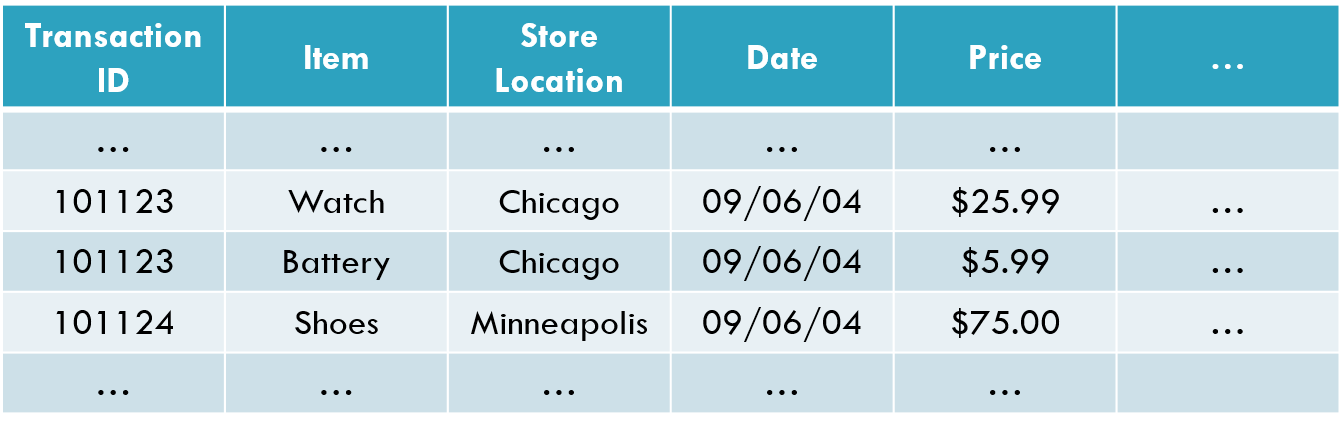
\includegraphics[width=0.8\linewidth,keepaspectratio]{aggred}
\end{center}
\end{frame}


%%%%%%%%%%%%%%%%%%%%%%%%%%%%%%%%%%%%%%%%%%%%%%%%%%%
\begin{frame}[fragile] \frametitle{Other Issues}
\begin{itemize}
\item Inconsistent Values Example:
	\begin{itemize}
	\item Data object with address, city, zip code in three separate fields
	\item But address / city is in a different zip code
	\end{itemize}
\item Some inconsistencies are easy to detect (and fix) automatically; others are not.
\item Duplicate Data Example:
	\begin{itemize}
	\item many people receive duplicate mailings because they are in a database multiple times under slightly different names
	\end{itemize}
\end{itemize}
\end{frame}


%%%%%%%%%%%%%%%%%%%%%%%%%%%%%%%%%%%%%%%%%%%%%%%%%%%
\begin{frame}[fragile] \frametitle{Other Issues}
\begin{itemize}
\item Timeliness:
	\begin{itemize}
	\item Data starts to age as soon as it has been collected
	\item Example: general population of users interact with Facebook differently than they did so 2 years ago
	\end{itemize}
\item Relevance:
	\begin{itemize}
	\item Sampling bias: occurs when a sample is not representative of the overall population
	\item Example: survey data describes only those who responded to the survey
	\end{itemize}
\end{itemize}
\end{frame}

%%%%%%%%%%%%%%%%%%%%%%%%%%%%%%%%%%%%%%%%%%%%%%%%%%%
\begin{frame}[fragile] \frametitle{When to Remove Variables}
\begin{itemize}
\item Variables that will not help the analysis should be removed:
	\begin{itemize}
	\item Unary variables: take on a single value Example: gender variable for students at an all-girls school
	\item Variables that are nearly unary Example: gender of football athletes at elementary school 99.95\% of the players are male
	\item Some data mining algorithms may treat the variable as unary Not enough data to investigate the female players anyway
	\end{itemize}
\item Think carefully before removing variables because of:
	\begin{itemize}
	\item 90\% of the values are missing
	\item Strong correlation between two variables
	\end{itemize}
\end{itemize}
\end{frame}


%%%%%%%%%%%%%%%%%%%%%%%%%%%%%%%%%%%%%%%%%%%%%%%%%%%
\begin{frame}[fragile] \frametitle{When to Remove Variables}
90\% of the values are missing:
\begin{itemize}
\item Are the values that are present representative or not?
\item If the present values are representative, then either (1) remove the variable or (2) impute the values.
\item If the present values are non-representative, their presence adds value.
\begin{itemize}
\item Scenario: donation\_dollars field in a self-reported survey
\item Assumption: those who donate a lot are more inclined to report their donation
\end{itemize}
\item Could also binarize the variable: donation\_flag
\end{itemize}

\end{frame}


%%%%%%%%%%%%%%%%%%%%%%%%%%%%%%%%%%%%%%%%%%%%%%%%%%%
\begin{frame}[fragile] \frametitle{When to Remove Variables}
 Strong correlation between two variables

\begin{itemize}
	\item Inclusion of correlated variables may ``double-count'' a particular aspect of the analysis, depending on the machine learning technique used.
	\item Example: precipitation and people on a beach
	\item Strategy \#1: remove one of the two correlated variables
	\item Strategy \#2: use PCA to transform the variables (beyond scope of course)
\end{itemize}
\end{frame}


%%%%%%%%%%%%%%%%%%%%%%%%%%%%%%%%%%%%%%%%%%%%%%%%%%%%
%\begin{frame}[fragile] \frametitle{OLAP and Multidimensional Data Analysis}
%
%		Whats important are the insights can be gained by looking at data from
%		a multidimentional viewpoint.
%		The starting point is usually a tabular representation of the data, such 
%		as a {\bf fact table}. 
%
%		Two steps are necessary in order to represent data as a multidimentional 
%		array:
%			\begin{enumerate}
%				\item identification of the dimensions
%				\item identification of an attribute that is the focus of the analysis.
%			\end{enumerate}
%
%		The values of an attribute seve as indices into the array for the dimension
%		corresponding to the attribute, and the number of attribute values in the size
%		of that dimension. 
%
%		The content of each cell represents the value of a {\bf taget quantity} that
%		we are interested in analyzing.
%
%\end{frame}
%
%%%%%%%%%%%%%%%%%%%%%%%%%%%%%%%%%%%%%%%%%%%%%%%%%%%%
%\begin{frame}[fragile] \frametitle{Analyzing Multidimensional Data}
%
%		The key motivation for taking a multidimensional viewpoiint of data is the 
%		importance of aggregating data in various ways. 
%
%		A multidimensional representation of the data, together with all possible totals
%		(aggregates), is known as a {\bf data cube}.
%		A data cube may have either more or fewer than three dimensions. A data cube
%		is a generalization of what is known in statistical terminology as a 
%		{\bf cross-tabulation}.
%
%		{\bf Dimensionality Reduction and Pivoting:}
%		\begin{itemize}
%			\item {\bf Aggregation} can be viewed as a form of aggregation.
%			\item{\bf Pivoting} refers to aggregating over all dimensions except two. The
%			result is a two-dimensional cross tabulation with the two specified dimensions
%			as the only remaining dimensions. 
%\end{itemize}
%
%\end{frame}
%
%
%%%%%%%%%%%%%%%%%%%%%%%%%%%%%%%%%%%%%%%%%%%%%%%%%%%%
%\begin{frame}[fragile] \frametitle{Slicing and Dicing}
%
%			\begin{itemize}
%				\item {\bf Slicing} is selecting a group of cells from the entire 
%				multidimensional array by specifying a specific value for one or more
%				dimensions.
%				\item {\bf Dicing} involves seleccting a subset of cells by specifying a 
%				range of attribute values. This is equivalent to defining a subarray
%				from the complete array. In practice, both operations can also be accompanied
%				by aggregation over some dimensions. 
%\end{itemize} 
%
%\end{frame}
%
%
%%%%%%%%%%%%%%%%%%%%%%%%%%%%%%%%%%%%%%%%%%%%%%%%%%%%
%\begin{frame}[fragile] \frametitle{Roll-Up and Drill-Down}
%
%			\begin{itemize}
%				\item Categories (attributes) can often be organized as a hierarchical tree or lattice.
%							\item For instance, years consist of months and weeks, both of which consist of days.
%							\item Locations can be divided into nations, which contains states, which in turn
%			contains cities. 
%							\item Likewise of products can be further subdivided. For example,
%			the product category, furniture, can be subdivided into the subcategories,
%			chairs, tables, sofas, etc. 
%							\item This hierarchical structure gives rise to  the 
%			roll-up and drill-down operations. 
%\end{itemize} 
%
%\end{frame}
%
%%%%%%%%%%%%%%%%%%%%%%%%%%%%%%%%%%%%%%%%%%%%%%%%%%%%
%\begin{frame}[fragile] \frametitle{Roll-Up and Drill-Down}
%
%			\begin{itemize}
%
%							\item To illustrate, starting with the original
%			sales data, which is a multidimensional array with entries for each date,
%			we can aggregate {\bf (roll-up)} the sales across all the dates in a month. 
%										\item Conversely, given a representation of the data where the times dimensions are
%			broken into months, we might want to split the monthly sales totals 
%			{\bf (drill-down)} into daily sales. 
%
%										\item Thus, roll-up and drill-down operations are related to aggregation. 
%										\item Notice, 
%			however, that they differ from the aggregation operations from last section
%because they aggregate cells within a dimension, not across the entire dimension. 
%\end{itemize} 
%\end{frame}
%
%%%%%%%%%%%%%%%%%%%%%%%%%%%%%%%%%%%%%%%%%%%%%%%%%%%%%%%%%%%
\begin{frame}[fragile]\frametitle{ML-based Approaches}
	\begin{itemize}
	\item Decision Tree/Random Forest
	\item Gives most important features
	\end{itemize}
\begin{lstlisting}
Features sorted by their score:
[(0.2321, 'fractal_dimension_mean'), (0.15359999999999999, 'concavity_worst'), (0.1164, 'radius_mean'), (0.088900000000000007, 'concave_points_sd_error'), (0.075999999999999998, 'perimeter_mean'), (0.062, 'texture_mean'), (0.0453, 'concave_points_worst'), (0.042599999999999999, 'area_sd_error'), (0.034200000000000001, 'symmetry_mean'), (0.024299999999999999, 'concave_points_mean'), (0.021399999999999999, 'fractal_dimension_worst'), (0.0207, 'radius_sd_error'), (0.015100000000000001, 'symmetry_worst'), (0.0086, 'smoothness_mean'), (0.0080999999999999996, 'fractal_dimension_sd_error'), (0.0077999999999999996, 'radius_worst'),\ldots, (0.0001, 'perimeter_worst')]
\end{lstlisting}

\end{frame}

%%%%%%%%%%%%%%%%%%%%%%%%%%%%%%%%%%%%%%%%%%%%%%%%%%%%%%%%%%%
\begin{frame}[fragile]\frametitle{Other Approaches}
	\begin{itemize}
	\item Principal Component Analysis (PCA)
	\item Independent Component Analysis (ICA)
	\item Self Organizing Maps (SOM)
	\item Auto Encoders
	\end{itemize}
\end{frame}


